\begin{center}
	\vspace{0.5cm}{\parbox{16cm}{\small{\centering{\textbf{Аннотация}\\
					\hspace{0.6cm} В этом отчёте изложены результаты выполнения лабораторной работы <<Измерение вращательной и колебательной температур в газовом разряде по спектру молекулы $N_2$>>. В данной работе значения вращательной и колебательной температур определяются по электронно-колебательно-вращательным спектрам
					излучения второй положительной системы азота. В качестве объекта исследования рассматривается тлеющий разряд в воздухе при давлении
					10-30 Тор, поддерживаемый в потоке газа между двумя электродами
					специальной конструкции.
				}}}}
\end{center}

\textbf{\emph{Цель работы:}} работа посвящена ознакомлению со спектральными методами измерения поступательной, вращательной и колебательной температур в газоразрядной плазме и приобретении навыков работы со
спектральными приборами. В описании излагается краткая теория формирования молекулярных спектров
в газоразрядной плазме на примере молекулы азота, дается краткий обзор различных методов измерения
температур в неравновесных условиях низкотемпературной плазмы. Рассматриваются методы измерения
вращательной температуры в газоразрядной воздушной плазме по неразрешенной вращательной структуре
излучения 0–0- полосы (2+)-системы азота и колебательной температуры по относительной интенсивности
электронно-колебательных полос (2+)-системы азота.
\section{Введение}
Низкотемпературная плазма газового разряда является неравновесной средой, в
которой значения поступательной, вращательной, колебательной и электронной
температур обычно заметно различаются. В данной работе значения вращательной и
колебательной температур определяются по электронно-колебательно-вращательным
спектрам излучения второй положительной системы азота. В качестве объекта
исследования рассматривается тлеющий разряд в воздухе при давлении 10-30 Тор,
поддерживаемый в потоке газа между двумя электродами специальной конструкции.
\subsection{Теоретическое введение}
В основе большинства источников света лежит газовый разряд – это прохождение тока через воздух или другой газ. Газ, имеющий высокую температуру и состоящий из заряженных и нейтральных частиц, называется плазмой. При самостоятельном газо-вом разряде между электродами всегда образуется плазма.
Основные свойства низкотемпературной плазмы как неравновесной среды являются результатом способа её поддержания. Электрическое поле, создаваемое путем прикладывания напряжения между электродами, ускоряет более подвижные электроны, которые затем передают свою энергию молекулам газа как при упругих, так и при неупругих соударениях. При характерных значениях электрического поля большая часть энергии электронов переходит в колебательную энергию молекул газа. Затем эта энергия может переходить в химическую энергию продуктов плазмохимических реакций, в излучение, а также за счет колебательно-поступательной релаксации — во вращательную и поступательную энергию молекул. На последней стадии сообщенное газу тепло передается стенкам разрядной камеры и электродам. В связи с этим в большинстве случаев выполняется следующее соотношение: 

\begin{equation}
T_e > T_{vib} > T_{rot} \approx T_{tr},
\end{equation}

где $T_e$-- электронная температура разряда, $T_{vib}$-- колебательная температура, $T_{rot}$-- вращательная температура , $T_{tr}$-- поступательная температура. В большинстве случаев вращательная и поступательная температуры близки.

В настоящей работе $T_{rot}$ и $T_{vib}$ определяются по электронно-колебательно-вращате
льным спектрам, соответствующим переходам второй положительной (2+)-системы азота. Переходы с изменением только вращательного чиста называются вращательными, с изменением колебательного числа — колебательно-вращательными, с изменением электронного состояния — электронно-колебательно-вращательными. Допустимые переходы между различными электронными состояниями подчинены некоторым правилам отбора:

\begin{enumerate}
	
	\item $\Delta \Lambda = 0, \pm 1 $ , 
	\item мультиплетность $2S+1$ не меняется,
	\item при изменении колебательного квантового числа выполняется принцип Франка-Кондона,
	\item при изменении вращательного квантового числа $\Delta J = 0, \pm 1 $, причем запрещен переход 0 $\rightarrow $ 0,
	\item для перехода $ \Sigma \rightarrow \Sigma $ выполняется $ \Delta J \neq 0$.	
\end{enumerate}

Зависимость интенсивности линии от колебательных чисел $\nu$' и $\nu$'' определяется заселенностью верхнего уровня $N(\nu')$, например, для распределения Больцмана с колебательной температурой $T_{vib}$

\begin{equation}
N' \sim \exp \left[ -\frac{G'(\nu)}{T_{vib}} \right]
\end{equation}

и величиной фактора Франка—Кондона. Согласно этому принципу, электронный переход проходит так быстро, что за время перехода межъядерное расстояние колеблющейся молекулы не успевает измениться. То есть переход совершается вертикально.

\begin{figure}[H]
	\begin{center}
		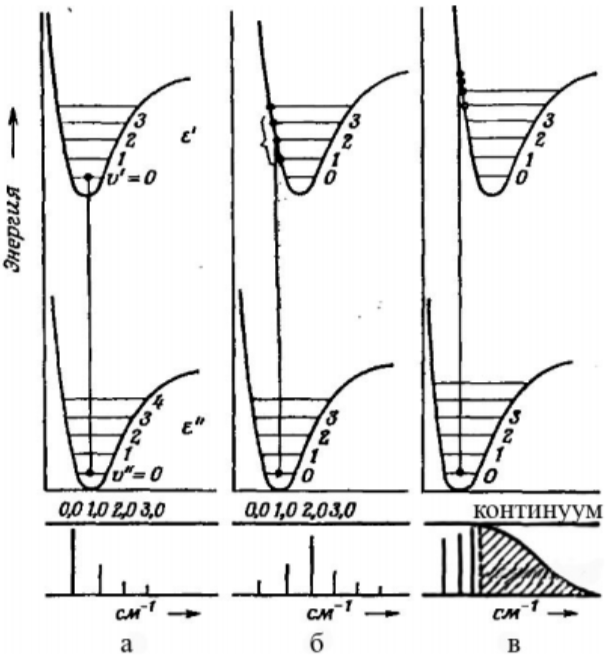
\includegraphics[width=0.49\textwidth]{fk.png}
		\caption{Демонстрация принципа Франка-Кондона}
	\end{center}	
\end{figure}

Из распределения Больцмана с колебательной температурой получаем зависимость интенсивности полос от колебательной температуры: 

\begin{equation}
\ln{\frac{I_{\nu' \nu ''}}{{\nu}_{\nu' \nu''}^4 q_{\nu' \nu''}}} = - \frac{G(\nu')}{0,6925T_{vib}} + C,
\end{equation}

где $G(\nu')$-- значения колебательной энергии в $\text{см}^{-1}$, $I_{\nu' \nu ''}$-- интенсивность излучения с колебательного уровня $\nu'$, $q_{\nu' \nu''}$-- коэффициент Франка-Кондона с данного перехода, ${\nu}_{\nu' \nu''}$-- частота излучения, С-- постоянная.

Значения коэффициентов Франка-Кондона приведены в таблице \ref{tab:frank-koeffs}.

\begin{table}[H]
	\centering
	\caption{Значения коэффициентов Франка-Кондона}
	\begin{tabular}{ | l | l | l | l | l | l | l | l | l | }
		\hline
		переход & $0 \rightarrow 0$ & $0 \rightarrow 1$ & $1 \rightarrow 2$ & $0 \rightarrow 2$ & $1 \rightarrow 3$ & $2 \rightarrow 3$ & $2 \rightarrow 4$ & $3 \rightarrow 5$ \\ \hline
		$q_{\nu' \nu''}$ & 0.4527 & 0.3291 & 0.2033 & 0.1462 & 0.1990 & 0.06345 & 0.1605 & 0.09426 \\ \hline
	\end{tabular}
	\label{tab:frank-koeffs}
\end{table}

Значения $G(\nu)$ для начальных колебательных уровней приведены в таблице \ref{tab:G_table}

\begin{table}[H]
	\centering
	\caption{Значения $G(\nu)$}
	\begin{tabular}{ | l | l | l | l | l | l | l | l | l | }
		\hline
		$\nu$ & 0 & 1 & 2 & 3 & 4 \\ \hline
		$G(\nu)$, см$^{-1}$ & 1016.7 & 3011.1 & 4951.9 & 6826.0 & 8607.2 \\ \hline
	\end{tabular}
	\label{tab:G_table}
\end{table}


\subsection{Методики измерения}
Для измерения вращательной температуры необходимо получить спектр 0 $\rightarrow $ 0 полосы ($2^+$)-системы молекулы азота в режиме неразрешенной вращательной структуры. После получения спектра необходимо найти десятичный логарифм от интенсивностей и построить график зависимости lgI от $\lambda$, выделить прямолинейный участок, найти тангенс угла наклона прямой и по рисунку \figref{scheme} определить значение вращательной температуры.
\begin{figure}[H]
	\begin{center}
		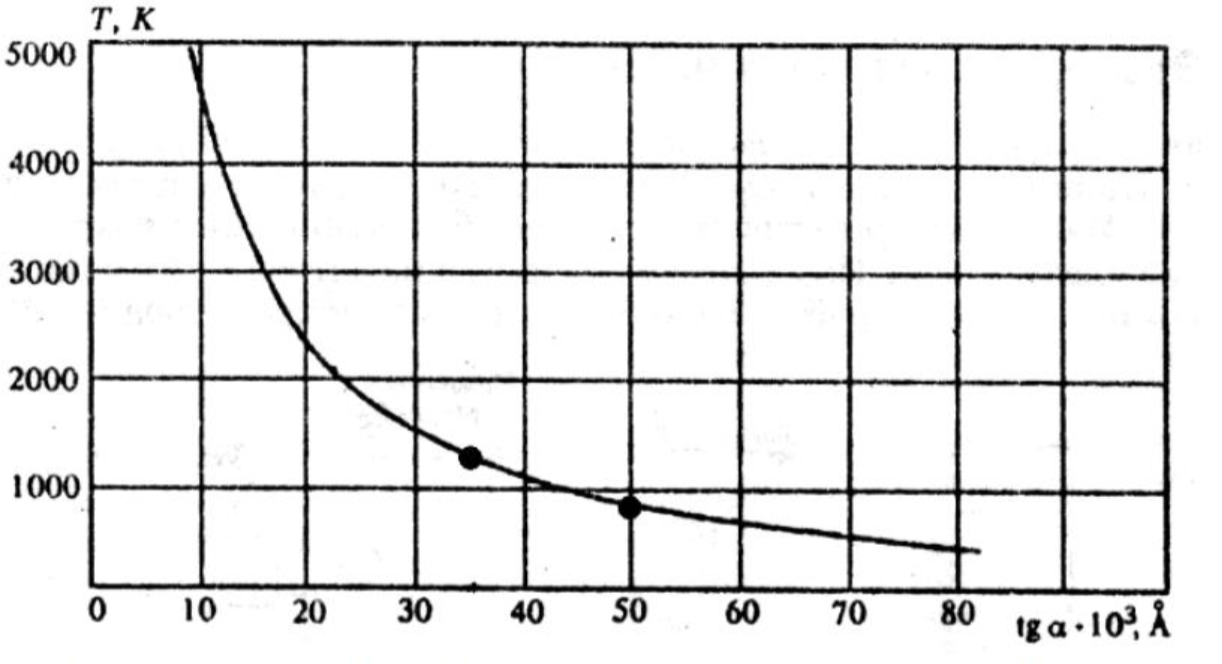
\includegraphics[width=0.65\textwidth]{kalibr.png}
		\caption{Калибровочный график для определения вращательной температуры}
		\label{scheme}
	\end{center}	
\end{figure}
Для измерения колебательной температуры необходимо записать спектры полос 0 $\rightarrow $ 1, 1 $\rightarrow $ 2, 0 $\rightarrow $ 2, 1 $\rightarrow $ 3 ($2^{+}$)-системы. Далее по формуле 3 определяем вращательную температуру.